%----------------------------------------------------------------------------------------
%	PACKAGES AND OTHER DOCUMENT CONFIGURATIONS
%----------------------------------------------------------------------------------------

\documentclass[paper=a4, fontsize=11pt]{scrartcl} % A4 paper and 11pt font size
\usepackage[a4paper, left=2.5cm, right=2cm, top=2cm, bottom=2cm]{geometry}
\linespread{1.2}

\usepackage[utf8]{inputenc}
\addtokomafont{disposition}{\rmfamily}
\usepackage{polski} % Język polski/hyphenation
\usepackage{amsmath,amsfonts,amsthm} % Math packages
\usepackage{indentfirst}
\usepackage{graphicx}
\usepackage{caption}
\usepackage{flafter}
\usepackage{flexisym}
\usepackage{listings}
\usepackage{color}


\def \thesis {Aplikacja uczenia maszynowego metodą SVM}
\def \author {Pavlo Boidachenko}
\def \department {Wydział Fizyki, Astronomii i Informatyki Stosowanej}

\usepackage{sectsty} % Allows customizing section commands
%\allsections{\mdseries\itshape} % Make all sections centered, the default font and small caps

\usepackage{fancyhdr} % Custom headers and footers
\pagestyle{fancy} % Makes all pages in the document conform to the custom headers and footers
\fancyhead[L]{\textbf{Praca licencjacka:} \thesis} % No page header - if you want one, create it in the same way as the footers below
\fancyhead[C]{}
\fancyhead[R]{}
\fancyfoot[L]{\author} % left footer
\fancyfoot[C]{\thepage} % center footer
\fancyfoot[R]{} % right footer
\renewcommand{\headrulewidth}{0.3pt} % Remove header underlines
\renewcommand{\footrulewidth}{0.3pt} % Remove footer underlines
\setlength{\headheight}{14.06pt} % Customize the height of the header

% bibliography
\usepackage[style=alphabetic,sorting=nyt,sortcites=true,autopunct=true,babel=hyphen,hyperref=true,abbreviate=false,backref=true,backend=biber,citestyle=numeric]{biblatex}
\addbibresource{ref.bib}
\defbibenvironment{bibliography}
  {\list
     {\printtext[labelnumberwidth]{%
      \printfield{labelprefix}%
      \printfield{labelnumber}}}
     {\setlength{\labelwidth}{\labelnumberwidth}%
      \setlength{\leftmargin}{\labelwidth}%
      \setlength{\labelsep}{\biblabelsep}%
      \addtolength{\leftmargin}{\labelsep}%
      \setlength{\itemsep}{\bibitemsep}%
      \setlength{\parsep}{\bibparsep}}%
      \renewcommand*{\makelabel}[1]{\hss##1}}
  {\endlist}
  {\item}

% listing settings
\definecolor{mygreen}{rgb}{0,0.6,0}
\definecolor{mygray}{rgb}{0.5,0.5,0.5}
\definecolor{mymauve}{rgb}{0.58,0,0.82}

\lstset{ 
  backgroundcolor=\color{white},   % choose the background color; you must add \usepackage{color} or \usepackage{xcolor}; should come as last argument
  basicstyle=\footnotesize,        % the size of the fonts that are used for the code
  breakatwhitespace=false,         % sets if automatic breaks should only happen at whitespace
  breaklines=true,                 % sets automatic line breaking
  captionpos=b,                    % sets the caption-position to bottom
  commentstyle=\color{mygreen},    % comment style
  extendedchars=true,              % lets you use non-ASCII characters; for 8-bits encodings only, does not work with UTF-8
  frame=single,	                   % adds a frame around the code
  keepspaces=true,                 % keeps spaces in text, useful for keeping indentation of code (possibly needs columns=flexible)
  keywordstyle=\color{blue},       % keyword style
  language=C++,                 % the language of the code
  morekeywords={*,...},            % if you want to add more keywords to the set
  rulecolor=\color{black},         % if not set, the frame-color may be changed on line-breaks within not-black text (e.g. comments (green here))
  showspaces=false,                % show spaces everywhere adding particular underscores; it overrides 'showstringspaces'
  showstringspaces=false,          % underline spaces within strings only
  showtabs=false,                  % show tabs within strings adding particular underscores
  stepnumber=2,                    % the step between two line-numbers. If it's 1, each line will be numbered
  stringstyle=\color{mymauve},     % string literal style
  tabsize=2,	                   % sets default tabsize to 2 spaces
  title=\lstname                   % show the filename of files included with \lstinputlisting; also try caption instead of title
}

\numberwithin{equation}{section} % Number equations within sections (i.e. 1.1, 1.2, 2.1, 2.2 instead of 1, 2, 3, 4)
\numberwithin{figure}{section} % Number figures within sections (i.e. 1.1, 1.2, 2.1, 2.2 instead of 1, 2, 3, 4)

\renewcommand{\thetable}{\Roman{table}}

\setlength\parindent{10pt} % Removes all indentation from paragraphs - comment this line for an assignment with lots of text

\newcommand{\horrule}[1]{\rule{\linewidth}{#1}} % Create horizontal rule command with 1 argument of height

\newcommand*{\captionsource}[2]{% caption with source for images
  \caption[{#1}]{%
      #1}
    %\\\hspace{\linewidth}%
    Źródło: #2%
  %
}

\newcommand{\norm}[1]{\left\lVert#1\right\rVert}

%Other packages
\usepackage{multirow}
\usepackage{url}
\usepackage{bm}
\usepackage{xcolor}
\definecolor{Black}{RGB}{0,0,0}
\definecolor{Red}{RGB}{255,0,0}
\definecolor{Blue}{RGB}{0,0,255}
\definecolor{Green}{RGB}{0,255,0}
\definecolor{Gray}{RGB}{45,45,45}
\definecolor{linkcol}{RGB}{57,0,155}
\usepackage[unicode, pdftex, colorlinks=true, urlcolor=Gray, linkcolor=Gray, citecolor=Gray]{hyperref}

\usepackage{tocloft}
\renewcommand{\cftsecleader}{\cftdotfill{\cftdotsep}}

\begin{document}

\thispagestyle{empty}
\begin{titlepage}
    \begin{center}
        \Large \textbf{Uniwersytet Jagielloński w Krakowie}\vspace{0.2cm}\\ \department\\
        \vspace*{1cm} 
        \vspace{3cm}
        \Large
        \textbf{\author}\\\vspace{0.5cm}
        \normalsize Nr albumu: 1124969\\
        \vspace{2cm}
        \Huge
        \textbf{\thesis}

        \vspace{1.5cm}
        \normalsize
        Praca licencjacka\\
        na kierunku informatyki\\ \vspace{0.15cm}
        \vfill
        \vspace{2cm}
        \begin{minipage}{1\textwidth}
            \begin{flushright}
                Praca wykonana pod kierunkiem\\
                dr Grzegorz Surówka\\
                Zakład Technologii Informatycznych 
            \end{flushright}
        \end{minipage}
        \vspace{2cm}
        \begin{center}
            Kraków 2019
        \end{center}
    \end{center}

\end{titlepage}

\newpage 
 \thispagestyle{empty}
\vspace{2.5cm}
\begin{flushleft}
\large \textbf{Oświadczenie autora pracy}\vspace{0.6cm}\\
\end{flushleft}

\noindent Świadom odpowiedzialności prawnej oświadczam, że niniejsza praca dyplomowa została napisana przeze mnie samodzielnie i nie zawiera treści uzyskanych w sposób niezgodny z obowiązującymi przepisami.\\

\noindent Oświadczam również, że przedstawiona praca nie była wcześniej przedmiotem procedur związanych z uzyskaniem tytułu zawodowego w wyższej uczelni.
\vspace{2cm}
\begin{center}
    \begin{tabular}{lr}
        ................................~~~~~~~~~~~~~~~~~~~~~~~~~~~~~~~~~~~~~~&
        .......................................... \\
        {~~~~Kraków, dnia} & {Podpis autora pracy~~~~}
    \end{tabular}
\end{center}
\vspace{5cm}
\begin{flushleft}
    \large \textbf{Oświadczenie kierującego pracą}
\end{flushleft}

\noindent Potwierdzam, że niniejsza praca została przygotowana pod moim kierunkiem i~kwalifikuje się do przedstawienia jej w postępowaniu o nadanie tytułu zawodowego.
\vspace{2cm}
\begin{center}
    \begin{tabular}{lr}
        ................................~~~~~~~~~~~~~~~~~~~~~~~~~~~~~~~~~~~~~~&
        ............................................ \\
        {~~~~Kraków, dnia} & {Podpis kierującego pracą~~}
    \end{tabular}
\end{center}
\vfill

\newpage
\tableofcontents

\newpage
\section{Wstęp} % SECTION
\subsection{Motywacja}
    \par W aktualne czasy temat Uczenia Maszynowego jest popularny\ref{fig:google-trends-ml} jak nigdy do tego. 
    Projekty z użyciem Uczenia Maszynowego pozwalają na tworzenie aplikacji które
    jeszcze 10 lat temu trudno było wyobrazić.

    \begin{figure}[h]
        \begin{center}
            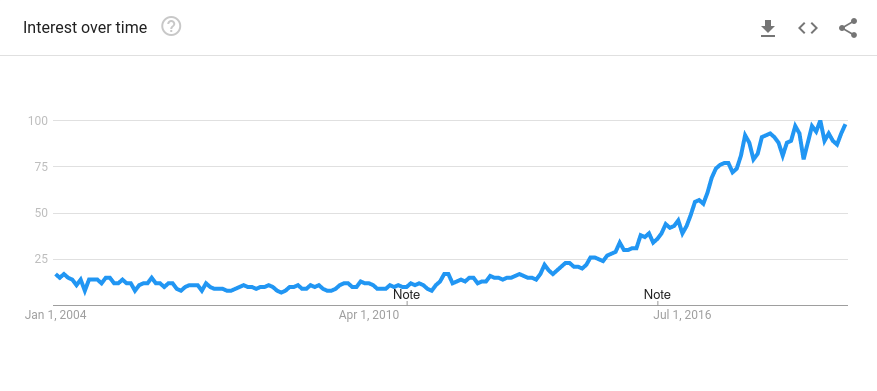
\includegraphics[scale=0.5]{./img/google-trends-ml.png}
            \captionsource{Machine Learning trends}{Google Trends}
            \label{fig:google-trends-ml}
        \end{center}
    \end{figure}

    \par Rozpowszechnienie Uczenia Maszynowego również spowodowało i moje zainteresowanie tematem.
    Z tego powodu dla swojej pracy licencjackiej wybrałem temat: Aplikacja uczenia maszynowego 
    metodą SVM.  Po zakończeniu pracy spodziewam się podwyższyć swoją kompetencje w dziale 
    Uczenia Maszynowego.

\subsection{Cel}
    \par Celem mojej pracy licencjackiej jest stworzenie oprogramowania pozwalającego na generowanie
    modeli używając Maszyny wektorów wspierających\textit{(ang. Support Vector Machine, SVM)} z graficznym 
    interfejsem użytkownika.  Program będą mogli użyć osoby potrzebujące szybko przetrenować kilka 
    modeli, przetestować ich dla różnych parametrów, zwizualizować dane. Program ma na celu ułatwienie
    pracę z Maszyną wektorów wspierających poprzez graficzny interfejs użytkownika
    oparty na bibliotekę QT. Część funkcjonalna programu jest oparta o bibliotekę LIBSVM\cite{CC01a}.

\subsection{Zakres}
    Program powinien móc ustawiać parametry dla wybranej metody oraz jądra\textit(ang. kernel), 
    generować wykresy podawanych zbiorów danych, interpretować różne formaty zbiorów danych, 
    wykonywać Sprawdzian krzyżowy (ang. Cross validation, CV), mieć metodę do optymalizacji 
    parametrów, pokazywać wyniki trenowania oraz testowania modeli.
\newpage

\section{Metoda klasyfikacji SVM} % SECTION
    \par W tym paragrafie w ogólnych zarysach jest opisana Maszyna Wektorów Wspierających
    oraz jej typy zaimplementowane w LIBSVM. Również będą krótkie opisy zaimplementowanych
    jąder.
\subsection{Opis}
    \par Swój program napisałem w oparciu o bibliotekę LIBSVM\cite{CC01a}. Maszyna Wektorów
    Wspierajacych(ang. Support Vector Machine. SVM) - klasyfikator, nauka którego ma na celu 
    wyznaczenie hiperpłaszczyzny rozdzielającej dwie klasy z maksymalnym marginesem. 
    Zaletą takiego klasyfikatora jest to że po uczeniu margines mówi jak dobrze są 
    odseparowane klasy. LIBSVM implementuje pięć typów Maszyny Wektorów Wspierajacych C-SVC, 
    $\nu$-SVC, One class SVM, $\epsilon$-SVR, $\nu$-SVR.
\subsection{C-SVC}
    \par C-Support Vector Classification - rodzaj klasyfikatora używający $C$ jako 
    parametr regularyzacji. Jeśli jest dany wektor $x_i \in R^n$, $i=1,...,l$ 
    w dwóch klasach i wektor etykiet $y_i \in \{1, -1\}$ to C-SVC rozwiązuję tak
    sformułowany problem:

    \begin{center}
        \begin{tabular}{rl}
            $\min\limits_{\pmb{\omega}, b, \varepsilon}$ & $\frac{1}{2} \pmb{\omega} ^T \pmb{\omega} +
            C \sum\limits_{i=1}^{l}\varepsilon_i$ \\
            Z zastrzeżeniem że & $y_i(\pmb{\omega}^T\phi(x_i) + b) \geq 1 - \varepsilon_i$ \\
                               & $\varepsilon_i \geq 0,i=1,...,l$
        \end{tabular}
    \end{center}

    \par Parametr $C$ służy do ustawienia marginesu: duży C $\rightarrow$ mały margines,
    mały C $\rightarrow$ duży margines.

    \begin{figure}[h]
        \begin{center}
            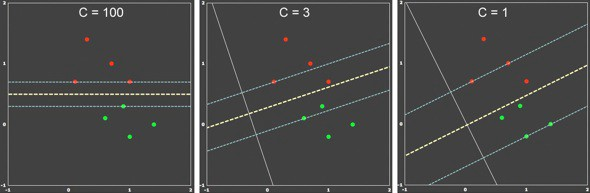
\includegraphics[scale=0.8]{./img/param_c.png}
            \captionsource{Zależność marginesu od parametru C}{\url{https://medium.com/@pushkarmandot}}
            \label{fig:param_c}
        \end{center}
    \end{figure}

    \par Dobry model dobrze separuję dane i razem z tym ma duży margines. Natomiast w
    w rzeczywistości jedno wyłącza drugie: duży margines włącza punkty z dwóch klas, a
    dobre separowanie może powodować przeuczanie(ang. Overfitting). Przeuczanie może 
    skutkować tym że model jest dobry na danych treningowych ale jest zły na danych testowych.

\newpage % description and equations was on different pages
\subsection{$\nu$-SVM}
    \par $\nu$-Support Vector Classification - rodzaj klasyfikatora używający $\nu$ jako
    parametr regularyzacji. Jest bardzo podobny do C-SVM, z różnicą że $\nu\in[0,1]$.
    Przyjemną właściwością $\nu$ jest to że on jest dolną granicą stosunku wektorów
    wspierających i górną granicą stosunku błędu uczenia.
    \par Jeśli jest dany wektor $x_i \in R^n$, $i=1,...,l$ w dwóch klasach i wektor
    $y\in R^l$ taki że $y_i \in \{1, -1\}$ to pierwotny problem optymalizacji wygląda
    następująco:

    \begin{center}
        \begin{tabular}{rl}
            $\min\limits_{\pmb{\omega},b,\varepsilon, \rho}$ &
            $\frac{1}{2}\pmb{\omega}^T\pmb{\omega} - \nu\rho + \frac{1}{l}\sum\limits_{i=1}^{l}
            \varepsilon_i$ \\
            Z zastrzeżeniem że & $y_i(\pmb{\omega}^T\phi(x_i) + b) \geq \rho - \varepsilon_i$ \\
                               & $\varepsilon_i \geq 0$, $i=1,...,l$, $\rho \geq 0$
        \end{tabular}
    \end{center}

\subsection{One-class SVM}
    \par One-class Support Vector Machine - rodzaj klasyfikatora uczenia
    nienadzorowanego, które zakłada brak etykiet w danych uczących. Ma na celu
    znalezienie niewiadomych wzorców/anomalii(klastrów) w danych wejściowych.  

    \begin{figure}[h]
        \begin{center}
            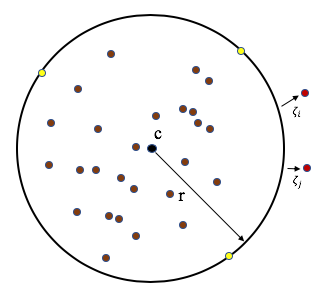
\includegraphics[scale=0.4]{./img/one-class-circle.png}
            \captionsource{Hipersfera zawierająca punkty danych. Ma środek c i promień R.
                            Punkty na krawędzi są wektorami wspierającymi.}{Wikipedia}
            \label{fig:one_class}
        \end{center}
    \end{figure}

    \par Jeśli dany jest wektor $x_i\in R^n$, $i=1,...,l$ bez informacji o klasach,
    to pierwotny problem optymalizacji wygląda następująco:

    \begin{center}
        \begin{tabular}{rl}
            $\min\limits_{\pmb{\omega},\varepsilon,\rho}$ & $\frac{1}{2}\pmb{\omega}^T\pmb{\omega} -
            \rho + \frac{1}{\nu l}\sum\limits_{i=1}^{l}\varepsilon_i$ \\
            Z zastrzeżeniem że & $\pmb{\omega}^T\phi(x_i)\geq\rho - \varepsilon_i$,\\
                               & $\varepsilon \geq 0$, $i=1,...,l$
        \end{tabular}
    \end{center}

\newpage
\subsection{$\epsilon$-SVR}
    \par Jeśli wektor etykiet $y_i \in R$ to jest używana metoda regresji.
    $\epsilon$-Support Vector Classification -  używa $C$ i $\epsilon$ jako
    parametrów regularyzacji. Celem jest znalezienie takiej funkcji $f(x)$
    że jej wartość odchyla się od $y_n$ na wartość nie większą od $\epsilon$
    dla każdego punktu z zbioru treningowego.
    \par Jeśli jest dany zbiór danych treningowych $\{(x_1, x_1),...,
    (x_l, z_l)\}$, gdzie $x-I \in R^n$ jest wektorem cech, a $z_i \in R^1$
    jest wyjściem. Przy danych parametrach $C>0$ i $\epsilon > 0$, standardowa 
    forma SVR to:

    \begin{center}
        \begin{tabular}{rl}
            $\min\limits_{\pmb{\omega},b,\pmb{\varepsilon}, \pmb{\varepsilon}^*}$ &
            $\frac{1}{2}\pmb{\omega}^T\pmb{\omega} + C\sum\limits_{i=1}^{l}
            \varepsilon_i + C\sum\limits_{i=1}^{l}\varepsilon_{i}^{*}$ \\
            Z zastrzeżeniem że & $\pmb{\omega}^T\phi(x_i) + b - z_i \leq \epsilon + \varepsilon_i$, \\
                           & $z_i - \pmb{\omega}^T\phi(x_i) - b \leq  \epsilon + \varepsilon_i^*$, \\
                           & $\varepsilon_i,\varepsilon_i^* \geq 0$,$i=1,...,l$

        \end{tabular}
    \end{center}

\subsection{$\nu$-SVR}
    \par $\nu$-Support Vector Regression - podobnie do $\nu$-SVC, używa parameter $\nu\in(0,1]$
    dla kontroli liczby wektorów wspierających. Również używa parametru $\epsilon$. Z parametrami
    $(C,\nu)$ $\nu$-SVR rozwiązuję:
    
    \begin{center}
        \begin{tabular}{rl}
            $\min\limits_{\pmb{\omega},b,\pmb{\epsilon},\pmb{\epsilon}^*,\epsilon}$ &
            $\frac{1}{2}\pmb{\omega}^T\pmb{\omega} + C(\nu\epsilon + \frac{1}{l}
            \sum\limits_{i=1}^{l}(\varepsilon_i+\varepsilon_i^*))$ \\
            Z zastrzeżeniem że & 
            $(\pmb{\omega}^T\phi(x_i) + b) - z_i \leq \epsilon + \varepsilon_i$,\\
           & $z_i - (\pmb{\omega}^T\phi(x_i) + b) \leq \epsilon + \varepsilon_i^*$,\\
           & $\varepsilon_i,\varepsilon_i^* \geq 0$, $i=1,...,l$, $\epsilon \geq 0$
        \end{tabular}
    \end{center}

\subsection{Jądra}
    \par W przypadku kiedy klasy nierozdzielne liniowo to jest używany trik z zastosowaniem
    funkcji jądrowych(ang. Kernel Trick). Funkcję jądrowe pozwalają odwzorować zbiór danych
    w przestrzeń z większą liczbą wymiarów, w której klasy danego zbioru będzie można rozdzielić
    hiperpłaszczyzną. 

    \begin{figure}[h]
        \begin{center}
            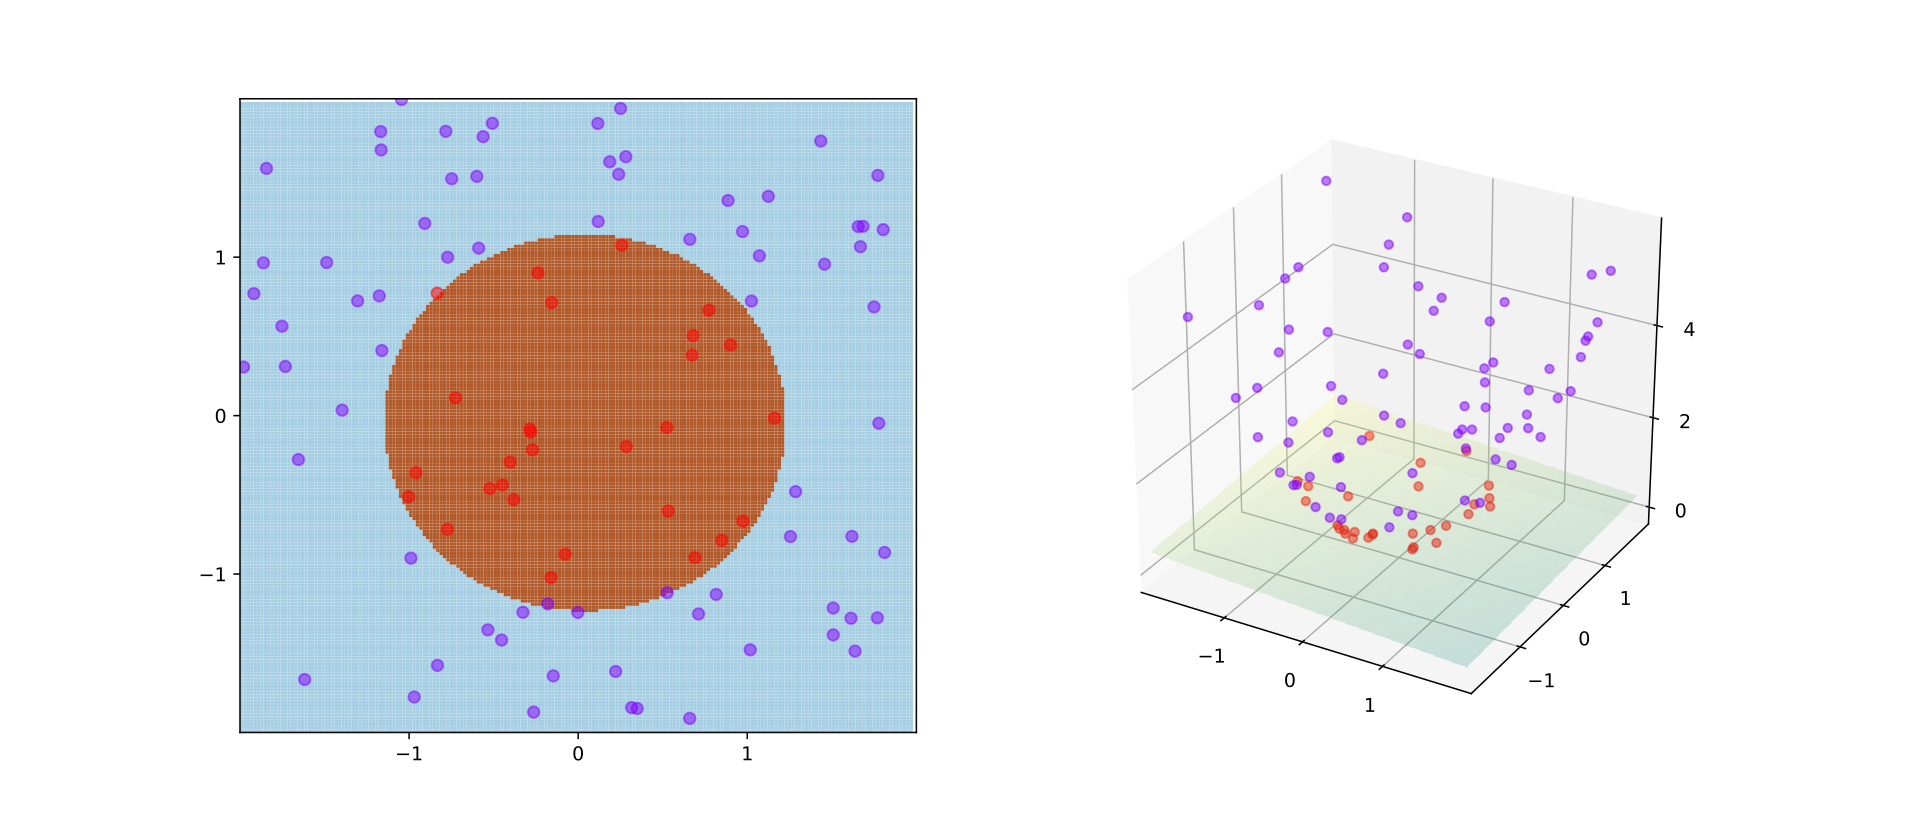
\includegraphics[scale=0.2]{./img/kernel_trick.png}
        \captionsource{Przykład stosowania funkcji jądrowej dla nierozdzielnego liniowo zbioru
        danych}{Wikipedia}
        \label{fig:kernel_trick}
        \end{center}
    \end{figure}

    \newpage 

    \par W bibliotece LIBSVM są zaimplementowane następne funkcje jądrowe:

    \begin{center}
        \begin{tabular}{rl}
            Liniowa & $K(x,x') = x\cdot x'$\\
            Wielomianowa & $K(x,x') = (\gamma*x \cdot x'+coef0)^{degree})$\\
            RBF & $K(x,x') =  -\gamma * (\sqrt{x}+\sqrt{x'}-2 * x\cdot x')$ \\
            Sigmoidalna & $K(x,x') = tanh(\gamma*x \cdot x'+coef0)$
        \end{tabular}
    \end{center}

    \par Autorzy biblioteki LIBSVM polecają \cite{hsu2003practical} że pierwsza funkcja jądrowa
    którą warto spróbować to RBF.  Jak pokazują \cite{keerthi2003asymptotic} jeśli używać RBF z
    optymalizacją hiperparametrów to nie ma potrzeby rozważać liniową funkcję jądrową. W sigmoidalnej
    funkcji jądrowej macierz jądrowa może nie być pozytywnie określona i generalnie dokładność modelu
    nie jest lepsza od RBF \cite{lin2003study}. 

\newpage
\section{Projekt aplikacji} % SECTION
    \par W tym paragrafie są opisane użyte technologie przy napisaniu aplikacji i interfejs
    użytkownika.

\subsection{Opis}
\subsection{Technologie}
    \par W roli jądra mojej aplikacji występuję biblioteka \textit{LIBSVM} napisana w 2011 roku
    przez Chih-Chung Chang i Chih-Jen Lin w Państwowym Uniwersytecie Tajwańskim. Celem autorów
    było zrobienie narzędzia z prostym interfejsem umożliwiające używanie Maszyny Wektorów
    Wspierajacych użytkownikom które nie zajmują się zawodowo nauczaniem maszynowym. Domyślnie
    użycie biblioteki \textit{LIBSVM} polega na skompilowaniu i używaniu dwóch programów:
    \textit{svm-train} i \textit{svm-predict}. \textit{svm-train} służy do trenowania modelu, 
    a \textit{svm-predict} do testowania, chociaż również może być używany do klasyfikacji
    nowych niegrupowanych danych. 

    \begin{figure}[h]
        \begin{center}
            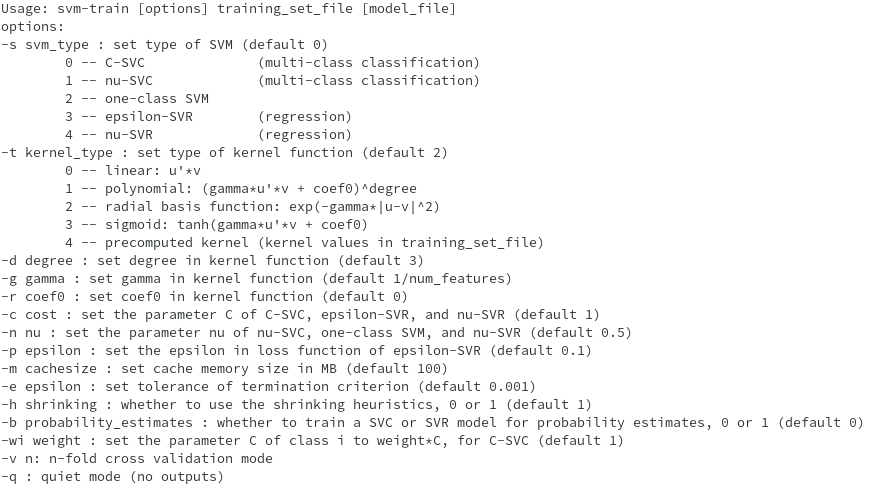
\includegraphics[scale=0.6]{./img/svm_train_usage.png}
            \caption{Użycie programu svm-train}
            \label{fig:train_usage}
        \end{center}
    \end{figure}

    \begin{figure}[h]
        \begin{center}
            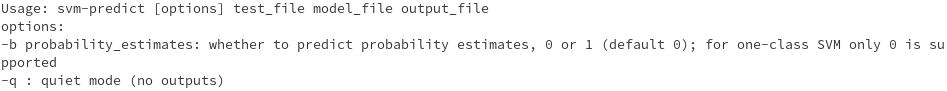
\includegraphics[scale=0.6]{./img/svm_predict_usage.png}
            \caption{Użycie programu svm-predict}
            \label{fig:predict_usage}
        \end{center}
    \end{figure}

    \par Aplikacja głównie jest napisana w języku \textit{C++}. Wybrałem ten język
    programowania przez jego wydajność mimo to że jest on językiem wysokiego poziomu. Na wybór
    \textit{C++} również wpłynęła moja sympatia do tego języka programowania, a napisanie
    dużego projektu w nim było dla mnie prawdziwym wyzwaniem, które pozwoliło pogłębić swoją
    wiedze w programowaniu i używaniu języka \textit{C++}.  Niektóre części aplikacji są
    napisane w języku Python, w szczególności te, które dotyczą rysowania wykresów, pracy z
    plikami i zmiennymi typu \textit{string}. Standardowa biblioteka Python przedstawia sporo
    narzędzi dla pracy z plikami i zmiennymi typu \textit{string}, co pozwala oszczędzać czas
    programisty w porównaniu do C++, w którym napisanie podobnej funkcjonalności zajęłoby o
    wiele więcej czasu. Dla rysowania wykresów użyłem biblioteki \textit{matplotlib}
    \cite{matplotlib} która pozwala stosunkowo łatwo rysować jedno, dwu i trzy-wymiarowe
    wykresy, a w kombinacji z \textit{numpy} i \textit{scipy} generować wykresy gęstości.
    \par Interfejs graficzny był pisany za pomocą biblioteki \textit{Qt}
    \cite{qtlibrary} napisanej w C++.  Twórcy biblioteki \textit{Qt} stworzyli IDE dedykowane
    do pracy z biblioteką - \textit{Qt Creator}. Jest ono wyposażone w szczegółową dokumentacje
    do biblioteki, wbudowany program \textit{Qt Designer} pozwala projektować interfejs
    graficzny metodą przeciągnij i upuść(ang. drag and drop), automatyczne uzupełnienie kodu,
    prowadzi analizę semantyczną kodu, wskazuje na błędy do kompilacji.  

\subsection{Interfejs użytkownika i realizacja funkcjonalności}
    \par Po uruchomieniu programu pierwsze co zobaczy użytkownik to okno główne. Po lewej
    stronie jest pole tekstowe w którym pojawiają się komunikaty o wynikach trenowania lub
    testowania modelu. W prawej górnej części okna są kontrolki do wybierania plików z danymi
    lub zapisywania pliku modelu. Żeby rozdzielić główną funkcjonalność od pobocznej i zrobić
    okno główne programu bardziej kompaktowym niektóre elementy są zrealizowane w postaci kart,
    natomiast funkcjonalność która dotyczy trenowania i testowania modelu jest
    dostępna bezpośrednio z okna głównego.

    \begin{figure}[h]
        \begin{center}
            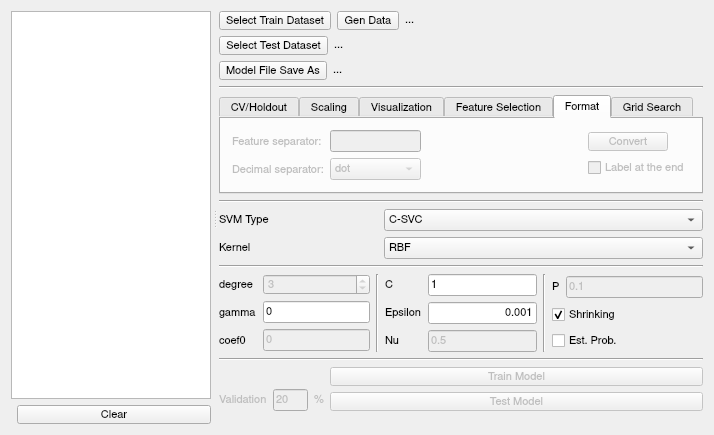
\includegraphics[scale=0.7]{./img/svm_app_main_window.png}
            \caption{Okno główne programu}
            \label{fig:main_window}
        \end{center}
    \end{figure}

\newpage % for better look
\subsubsection{Realizacja funkcjonalności głównej}
    \begin{enumerate}   

    \item Pole tekstowe dla komunikatów.

    \begin{figure}[h]
        \begin{center}
            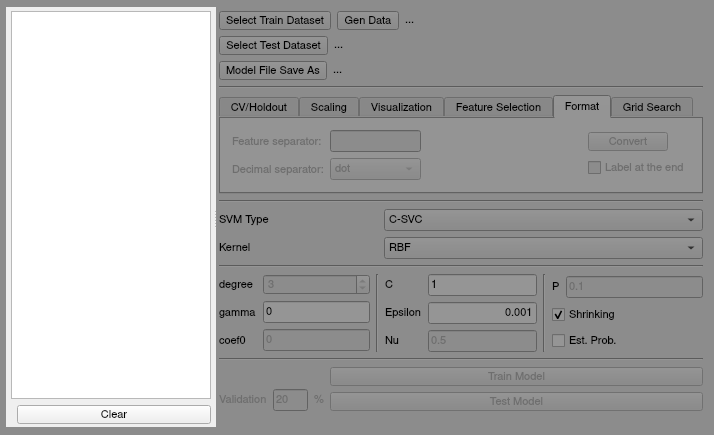
\includegraphics[scale=0.7]{./img/svm_app_mainw_textedit.png}
            \caption{Pole dla komunikatów}
            \label{fig:text_edit}
        \end{center}
    \end{figure}

    \par Dane pole tekstowe przyznaczone dla wypisywania komunikatów z biblioteki
    \textit{LIBSVM} lub używanych skryptów Python. W zasadzie opisywana kontrolka jest
    widżetem biblioteki \textit{Qt} \textit{TextEdit} w którym jest wyłączona możliwość
    edytowania zawartości. Dla tego żeby nie przerabiać kodu żródłowego biblioteki
    \textit{LIBSVM} zamieniając każde wywołanie funkcji \textit{printf} na odpowiednią funkcje,
    któraby dodawała tekst na \textit{TextEdit}, szukałem sposobu na przekierowanie całego
    wyjścia aplikacji na widżet w interfejsie graficznym. Niestety biblioteka \textit{Qt} nie
    przedstawia prostej możliwości na zrobienie tego, więc musiałem zraimplementować podobną
    funkcjonalność samodzielnie. Za tą funkcjonalność odpowiada klasa \textit{OutputHandler},
    która w swoim konstruktorze tworzy potok do którego przekierowuje \textit{stdout}.

    \begin{lstlisting}
    OutputHandler::OutputHandler()
    {
        _saved_stdout = dup(STDOUT_FILENO);
        pipe(_stdout_pipe);
        dup2(_stdout_pipe[1], STDOUT_FILENO);
        close(_stdout_pipe[1]);
    }
    \end{lstlisting}

    \par Za tym uruchamia wątek który ciągle sprawdza czy coś było zapisane do potoku i jeśli
    tak to wywołuje sygnał który dopisuje te dane do \textit{TextEdit} na interfejsie graficznym.

    \newpage
    \begin{lstlisting}
    void OutputHandler::handleOutput()
    {
        int bytes_read;
        char buf[1024];
        while((bytes_read = (int)read(_stdout_pipe[0], buf, sizeof(buf))))
        {
            emit updateOutput(QString::fromLatin1(buf, bytes_read));
            if(_cmd_out)
            {
                write(_saved_stdout, buf, bytes_read);
            }
        }
    }
    \end{lstlisting}

    \par Takie podejście pozwala używać standardowe sposoby na wypisywanie komunikatów i nie
    myśleć o tym czy wypisywany komunikat zostanie wyświetlony na interfejsie użytkownika.
    \par Pod omawianym polem tekstowym znajduje się przycisk \textit{Clean}, który usuwa
    wszystkie wcześniej wypisane komunikaty z pola \textit{TextEdit}. 

    \item Zarządzanie plikami z danymi

    \par Pierwszym krokiem który będzie musiał zrobić użytkownik po uruchamianiu aplikacji -
    wybrać plik z danymi dla trenowania. Dla tego celu na ekranie głównym są odpowiednie
    kontrolki które pozwalają wybrać plik z danymi do trenowania lub testowania i wybrać
    katalog w którym należy zapisać plik z wygenerowanym modelem. Domyślnie plik modelu ma
    nazwę [nazwa pliku z danymi do trenowania + .model]. Przycisk \textit{Gen Data} pozwala
    wygenerować plik z danymi samodzielnie, jego funkcjonalność będzie omówiona później.

    \begin{figure}[h]
        \begin{center}
            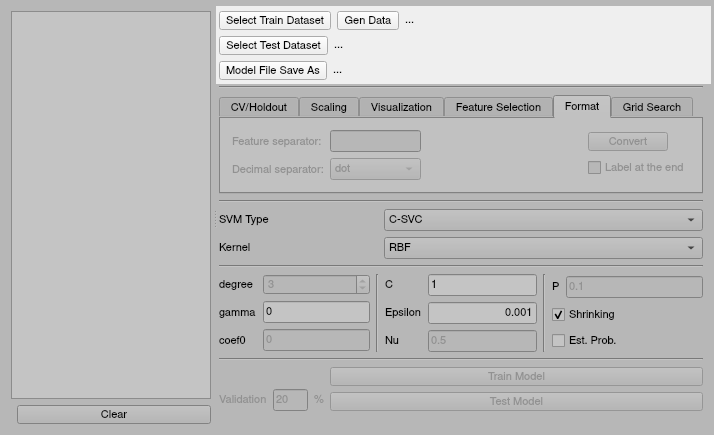
\includegraphics[scale=0.7]{./img/svm_app_mainw_filehandler.png}
            \caption{Zarządzanie plikami}
            \label{fig:file_handler}
        \end{center}
    \end{figure}

    \par Po wybraniu pliku z danymi program sprawdza czy dane są zapisane w formacie
    \textit{LIBSVM}. W przypadku poprawności danych program parsuje plik wypisując liczbę
    rekordów, liczbę klas i liczbę cech jak dla danych trenujących tak i dla danych testowych.

    \begin{figure}[h]
        \begin{center}
            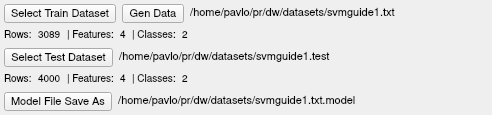
\includegraphics[scale=0.7]{./img/svm_app_mainw_filehandler_ex.png}
            \caption{Przykład wczytanych danych}
            \label{fig:files_example1}
        \end{center}
    \end{figure}

    \end{enumerate}

\newpage
\section{Podsumowanie} % SECTION
\subsection{Odniesienie do celu pracy}
\subsection{Co można dodać}

\newpage
\nocite{*}
\printbibliography

\end{document}
